\documentclass{article}
\usepackage{lipsum} % for placeholder text
\usepackage{graphicx}

\title{Handwritten Optical Character Recognition Project Report}
\author{Xinyu Meng, Zijie Li}
\date{\today}

\begin{document}

\maketitle

\section{abstract}
Handwritten Optical Character Recognition (OCR) presents a formidable challenge in the field of computer vision and artificial intelligence due to the variability and complexity of human handwriting. The goal of our project is to develop an OCR system capable of accurately recognizing handwritten text from various sources and formats. This system aims to bridge the gap between analog and digital text, enhancing accessibility and efficiency in document processing, archival, and retrieval. By leveraging advanced machine learning and deep learning techniques, our project seeks to surpass existing benchmarks in handwritten OCR accuracy and processing speed.
The objective of this project is to develop a robust OCR system capable of accurately recognizing handwritten characters from scanned documents or images. The proposed system will involve several stages including preprocessing, feature extraction, and classification. Preprocessing techniques such as binarization, noise reduction, and normalization will be applied to enhance the quality of input images. Feature extraction will be performed using CNNs, which will automatically learn discriminative features from the input images. The CNN architecture will be designed to effectively capture spatial dependencies and patterns inherent in handwritten characters.

\section{Introduction}
Handwritten OCR is a critical technology with applications ranging from historical document digitization to automating form processing. Despite advancements in OCR technology, the recognition of handwritten text remains a challenge due to its inherent variability. Our project proposes to address this challenge by developing a robust model that combines convolutional neural networks (CNNs) with recurrent neural networks (RNNs), specifically Long Short-Term Memory (LSTM) networks, to effectively learn and predict sequences of handwritten characters.

\section{Related Work}

\begin{itemize}
\item Learning to Extract Semantic Structure from Documents Using Multimodal Fully Convolutional Neural Network. ,Yang, X., Yumer, E., Asente, P., Kraley, M., Kifer, D., \& Giles, C. L. CVPR 2017

\item Sequence to sequence learning with neural networks. Sutskever, I., Vinyals, O., \& Le, Q. V. NIPS 2014

\item Cnn-n-gram for handwriting word recognition. Poznanski, A., \& Wolf, L.CVPR 2016
Reading text in the wild with convolutional neural networks. Jaderberg, M., Simonyan, K., Vedaldi, A., \& Zisserman, A. (IJCV 2016

\end{itemize}

\section{OCR Model Architecture}

The Optical Character Recognition (OCR) model used in this project is based on a Convolutional Neural Network (CNN) combined with a Recurrent Neural Network (RNN) using Long Short-Term Memory (LSTM) units. The architecture of the model can be summarized as follows:

\begin{itemize}
    \item \textbf{Input Layer}: The input images are of shape (32, 128, 1), representing a height of 32 pixels and a width of 128 pixels with a single channel for grayscale.
    
    \item \textbf{Convolutional Layers}: Several convolutional layers with different filter sizes are used to extract features from the input images. These layers are followed by activation functions such as ReLU and Batch Normalization to introduce non-linearity and improve convergence.
    
    \item \textbf{Pooling Layers}: Max-pooling layers are applied to downsample the feature maps and reduce the spatial dimensions while retaining important features.
    
    \item \textbf{Recurrent Layers}: Bidirectional LSTM layers are employed to capture the temporal dependencies in the sequential data of the extracted features. This allows the model to learn patterns and relationships between characters in the text.
    
    \item \textbf{Output Layer}: The output layer consists of a softmax activation function that predicts the probability distribution over the character classes, including alphanumeric characters, punctuation marks, and special symbols.
\end{itemize}

\begin{figure}
    \centering
    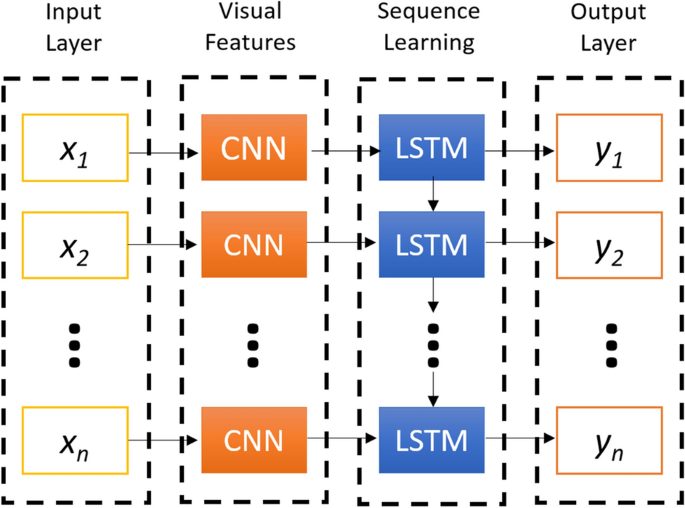
\includegraphics[width=0.5\linewidth]{41598_2021_93656_Fig2_HTML.png}
    \caption{CNN-LSTM model structure}
    \label{fig:enter-label}
\end{figure}

\section{IAM Handwriting Database}

The IAM Handwriting Database is a widely used benchmark dataset in the field of handwritten text recognition. It consists of handwritten text samples collected from forms, letters, and other documents. We've excluded the error-labeled words for training purpose. The dataset is structured as follows:

\begin{itemize}
    \item \textbf{Text Samples}: The dataset contains 1'539 pages of scanned text, 115'320 isolated and labeled words.
    
    \item \textbf{Ground Truth Labels}: Each word sample in the IAM dataset is accompanied by ground truth labels that provide the correct transcription of the handwritten text.
    
    \item \textbf{Variety of Writing Styles}: The IAM dataset includes english word samples written in various writing styles, sizes, and orientations, making it a diverse and challenging dataset for OCR tasks.
    
    \item \textbf{Data Preprocessing}: Before training our OCR model on the IAM dataset, we perform several preprocessing steps to enhance the quality of the handwritten text samples with opencv. These preprocessing steps include image conversion/reshaping, enhancement, grayscale, segmentation, normalization, and train/test split.
\end{itemize}


\section{Results}

After training and evaluating our OCR model on the IAM Handwriting Database and other relevant datasets, we achieved promising results in terms of accuracy, performance, and generalization. The following subsections outline the key results obtained from our experiments:

\subsection{Accuracy Metrics}

Using 5000 records with 4000 training data, we evaluated the accuracy of our OCR model using standard metrics. The results indicate that our model achieved a high accuracy rate in accurately transcribing handwritten text from scanned documents. The training accuracy increased from 0 to 98.59 in the 30 epochs we trained. While using 500 records, the model can reach 7.32 accuracy and loose is 12.031. On validation with jaro-winkler, our score is 90.39. 

\begin{figure}
    \centering
    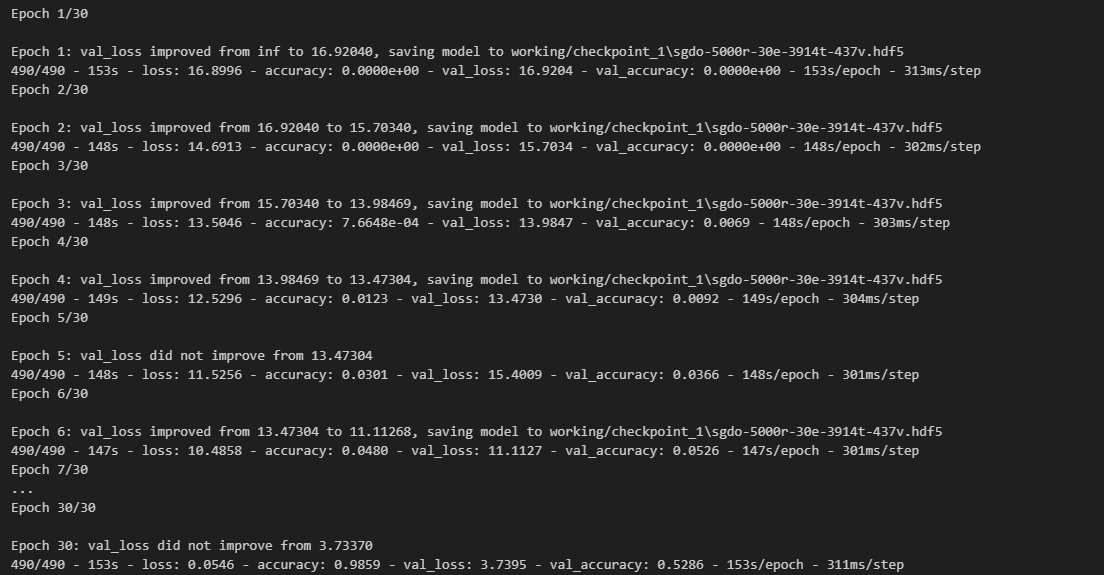
\includegraphics[width=1\linewidth]{image.png}
    \caption{Training Result}
    \label{fig:enter-label}
\end{figure}

\subsection{Performance Evaluation}

In addition to accuracy, we assessed the performance of our OCR model in terms of speed, scalability, and resource utilization. When running the model from local machine, it takes around 1.5 hour to train on 4000 records. 


\subsection{Generalization and Robustness}

We tested the generalization and robustness of our OCR model by evaluating its performance on challenging handwriting styles. The model exhibited robustness in handling diverse text samples and maintained high accuracy across different scenarios.

\subsection{Application Scenarios}

Finally, we discussed potential application scenarios and use cases where our OCR model can be deployed effectively, such as document digitization, text extraction, and archival purposes.

\begin{figure}
    \centering
    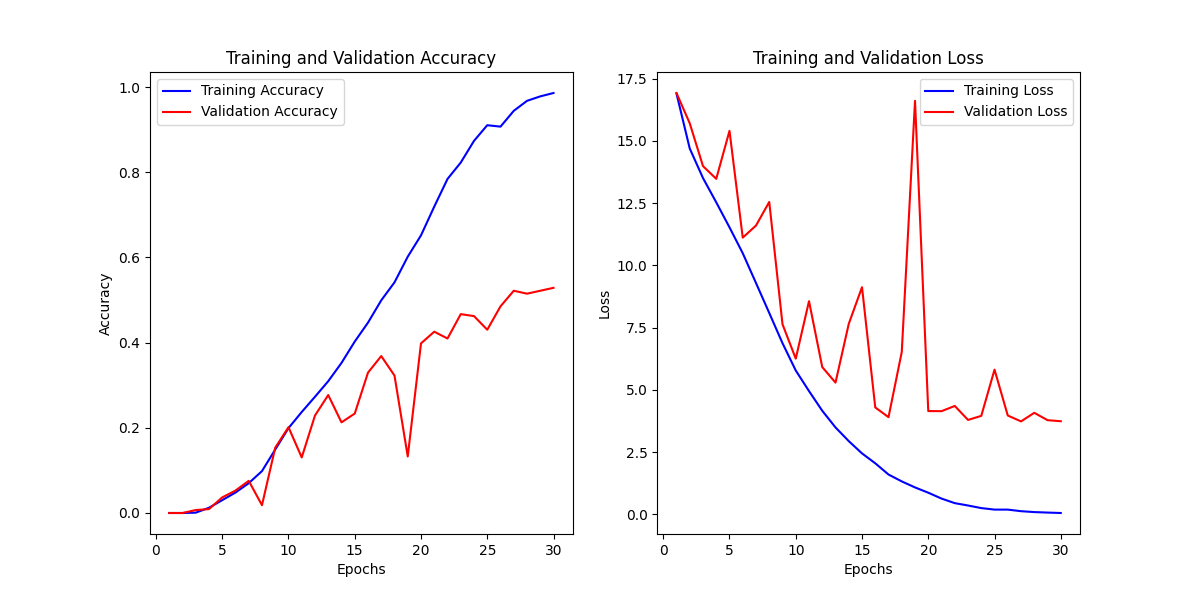
\includegraphics[width=1\linewidth]{Accuracy_Loss_Plot.png}
    \caption{Model Accuracy and Loss}
    \label{fig:loss}
\end{figure}


\section{Limitations}

While our OCR model has shown promising results, the performance of our OCR model may degrade when dealing with noisy or low-quality images, specifically, when dealing with the err words in the IAM dataset, the accuracy can be low.

While our OCR model supports recognition of English text, it may not be optimized for other languages or character sets. Expanding language support and multilingual capabilities can broaden the applicability of the OCR system to diverse linguistic contexts. The computational resources required for training and deploying our OCR model, especially in deep learning architectures like CNN-LSTM, can be substantial. It could take 2-3 hours to train on full length of the IAM dataset.

\section{Conclusions}

In this project, we developed a hybrid CNN-LSTM architecture for Handwritten Optical Character Recognition (OCR) and evaluated its performance on the IAM Handwriting Database. Our key findings and conclusions are as follows:
The OCR model achieved competitive accuracy rates on IAM datasets, demonstrating its effectiveness in recognizing handwritten text from scanned documents or images. The combination of Convolutional Neural Networks (CNNs) for feature extraction and Long Short-Term Memory (LSTM) networks for sequence modeling proved to be a robust approach for OCR tasks.
Our model exhibited robustness to variations in handwriting styles, achieving reliable performance across a diverse range of writing samples in the IAM database. 

\section{Individual Contributions}

\begin{itemize}
    \item {Xinyu Meng}: Conducting comprehensive research on OCR techniques, deep learning models, and dataset selection. Researching referencing from the internet about the implementation detail for the hybrid CNN-LSTM architecture. Collaborating with team members on data analysis, result interpretation, and performance evaluation. Writing and documenting the github repository, ensuring readability, modularity, and adherence to best practices. Drafting sections of the project report, including the methodology, results, and conclusions.
    \item {Zijie Li}: Structured the project proposal and abstract. Researching and selecting appropriate datasets for training and testing the OCR model. Implementing data preprocessing techniques. Collaborating with team members on model architecture design, experimentation, and performance evaluation. Conducting extensive experiments to fine-tune hyperparameters, optimize training strategies, and improve model convergence. Assisting in result analysis, visualization. Contributing to the project documentation, and constructing the presentation slides. 
\end{itemize}

\end{document}
